% ============================================================
% CANOPI — Neural Processing Letters submission (Springer sn-jnl).
% Self-contained: % ============================================================
% Related Work — NPL resubmission. Concedes prior canonicalization work
% up front, then stakes the delta. \cite keys are in references_npl.bib.
% ============================================================
\section{Related Work}\label{sec:related}

\subsection{Prompt injection and neural guardrails}
Prompt injection is the top-ranked vulnerability for LLM applications
(OWASP LLM01)~\cite{owasp2025}, spanning direct injection in user input and
indirect injection smuggled through retrieved context or tool output.
A now-standard mitigation is a \emph{neural guardrail}: a transformer classifier
trained to flag injection or jailbreak content before it reaches the model.
Representative open detectors include ProtectAI's DeBERTa-based
classifier~\cite{protectai2024}, InjecGuard~\cite{injecguard2024}, and
PromptGuard~\cite{promptguard2025}; Meta's Prompt Guard~2 reports $97.5\%$ recall
at a $1\%$-FPR operating point in-distribution~\cite{metapromptguard2}, the bar our
method must match. These detectors are typically evaluated by
aggregate ranking metrics (AUROC) on clean, English, in-distribution test sets,
which---as we show in Section~\ref{sec:results}---obscures their behavior under
both adversarial obfuscation and the low-false-positive operating points that
deployments require.

\subsection{Character-level obfuscation attacks}
A growing body of red-team work shows that trivial, meaning-preserving character
perturbations evade production guardrails. Homoglyph substitution (e.g., Cyrillic
\foreignlanguage{russian}{а} U+0430 for Latin \texttt{a}) reaches attack-success
rates of 42--59\% against open models~\cite{elastic2025homoglyph}; invisible
zero-width and Unicode-tag characters, and emoji variation-selector smuggling,
fully bypass several commercial shields including ProtectAI~v2 and Azure Prompt
Shield~\cite{mindgard2025invisible,csa2026unicode}. Crucially, the LLM tokenizer
typically reconstructs the intended semantics, so the attack changes the
classifier's input distribution without changing meaning---a covariate shift we
formalize in Section~\ref{sec:method}.

\subsection{Canonicalization as a defense---and our delta}
Input normalization is \emph{not} a new defensive idea, and we state this plainly.
NFKC normalization, zero-width stripping, and confusable folding as a
prompt-injection mitigation appear in recent work~\cite{llmsec2025bypass}, in
open-source tooling~\cite{cleanrepo}, and in a granted patent on Unicode
canonicalization of prompt injections~\cite{patent2025canon}; a
normalization-aware shield lowers average homoglyph exposure from 94.1\% to
43.9\%~\cite{llmsec2025bypass}. Related input-transformation defenses---spotlighting
and datamarking of untrusted spans~\cite{hines2024spotlighting} and
paraphrase/retokenization~\cite{jain2023baseline}---likewise operate at the
orthographic or structural level and address neither semantic nor cross-lingual
paraphrase. Our contribution is therefore \emph{not} the idea
of canonicalizing input. It is fourfold: \textbf{(i)} a \emph{detector-agnostic}
evaluation that quantifies recall recovery at a fixed 1\%-FPR operating point
across structurally different detectors, surfacing an under-reported
\emph{over-trigger counter-case} (a detector whose recall \emph{rises} under
obfuscation, so canonicalization normalizes rather than restores it);
\textbf{(ii)} an \emph{adaptive-adversary} evaluation that locates where
canonicalization is evaded (out-of-map confusables, tag-character smuggling) and
shows a hardened canonicalizer closing those gaps, answering the
``attacker-moves-second'' critique~\cite{attackersecond2025}; \textbf{(iii)} a
unification of \emph{character} and \emph{linguistic} canonicalization, extending
the same pre-classifier to cross-lingual and romanized-Arabic injection; and
\textbf{(iv)} a principled \emph{taxonomy}---canonicalization provably neutralizes
information-preserving perturbations and provably cannot neutralize semantic ones.

\subsection{Adaptive robustness}
Static defenses are routinely broken by adversaries who adapt to
them~\cite{attackersecond2025}. Most canonicalization studies report only static
attacks. We therefore evaluate against an adversary aware of the canonicalization
stage and report the defense's \emph{envelope} rather than a single headline.

\subsection{Multilingual and romanized injection}
Safety alignment is English-dominant, so translated prompts---not only in
low-resource languages---evade guardrails far more
often~\cite{yong2023lowresource,deng2024multilingual,babel2025}. The remedies
proposed so far are \emph{model-side}: multilingual safety
fine-tuning~\cite{deng2024multilingual} or LLM-based reasoning
guardrails~\cite{mrguard2025,sealguard2025} that place a generative model in the
inference path. To our knowledge no lightweight, no-LLM \emph{detector} recovers
cross-lingual detection at a fixed low-FPR operating point---the gap CANOPI closes
(Section~\ref{sec:results}). Romanized Arabic (Latin-script Arabic)
and Arabic transliteration are documented \emph{jailbreak vectors}~\cite{arabizi2024};
romanized-to-Arabic transliteration is itself an established NLP
task~\cite{wanlp2020arabizi}. To our knowledge the \emph{defensive} use of
transliteration-plus-translation as a canonicalization stage against
romanized/code-switched injection is unexplored, and is a contribution unique to
this work.

\subsection{Learned representations and operating-point objectives}
Closest to our learned component are detectors that train a representation to
separate benign from malicious inputs. Supervised contrastive
learning~\cite{khosla2020supcon} underpins recent jailbreak detectors; the most
similar, concurrent work fits a lightweight contrastive projection over a frozen
backbone~\cite{rcs2025}, but in the vision--language setting, with neither a
cross-lingual component nor an explicit low-false-positive objective. Such methods
optimize \emph{average} separation (AUROC) and reach a strict operating point, if
at all, only by \emph{post-hoc} threshold calibration. Optimizing the low-FPR
region \emph{directly}---partial-AUC and ``accuracy-at-the-top''
surrogates~\cite{macha2020deeptoppush,zhu2022pauc}---is well studied in
classification but, to our knowledge, has never been applied to prompt-injection
or jailbreak detection. CANOPI couples this operating-point objective to a
multi-view, cross-lingual intent-invariance term on top of the frozen orthographic
canonicalizer, training only a projection head with \emph{no} generative model in
the inference path---unlike LLM-based guardrails~\cite{mrguard2025} or
LLM-as-judge pipelines. The resulting property is one none of the above provides:
recovery of cross-lingual recall \emph{at a fixed $1\%$-FPR threshold}. Following
the adaptive-evaluation norm~\cite{carlini2019eval,attackersecond2025}, and
consistent with broader guardrail evaluations~\cite{sok2025guardrails}, we report
recall against an adaptive semantic-rewrite adversary rather than a single static
number, and disclose the residual our canonicalization provably cannot remove.
; all other sections inline.
% Primary result (monolingual mechanism) is final 5-seed; sections marked
% [PROVISIONAL] use the smoke pass pending the full 5-seed multilingual run.
% ============================================================
\documentclass[pdflatex,sn-mathphys-num]{sn-jnl}

\usepackage{graphicx}%
\usepackage{multirow}%
\usepackage{amsmath,amssymb,amsfonts}%
\usepackage{amsthm}%
\usepackage{mathrsfs}%
\usepackage[title]{appendix}%
\usepackage{xcolor}%
\usepackage{textcomp}%
\usepackage{booktabs}%
\usepackage{float}%
\usepackage{hyperref}%

\newcommand{\Rfpr}{\textrm{R@1\%FPR}}
\newcommand{\canon}{c}
\theoremstyle{plain}
\newtheorem{proposition}{Proposition}

\raggedbottom

\begin{document}

\title[Cross-Lingual Invariance as a Substitute for Multilingual Pretraining]{CANOPI: A Cross-Lingual Invariance Objective for Prompt-Injection Detection that Substitutes for Multilingual Pretraining}

\author*[1]{\fnm{Shaikhah} \sur{Alkhadhr}\orcidID{0000-0001-5938-2953}}\email{s.alkhadhr@ku.edu.kw}
\author[1]{\fnm{Heba} \sur{Alturki}\orcidID{0009-0004-4220-7947}}\email{h.alturki@ku.edu.kw}
\author[1]{\fnm{Aseel} \sur{Alqemlas}\orcidID{0009-0005-3960-7074}}\email{aseel.a8@ku.edu.kw}

\affil*[1]{\orgdiv{Information Science Department}, \orgname{Kuwait University},
\orgaddress{\street{Sabah AlSalem University City}, \city{Safat}, \postcode{13060},
\state{Al-Shadadiya}, \country{Kuwait}}}

% ============================================================
\abstract{
Neural guardrails are the dominant defense against prompt injection in
LLM-integrated applications, but they are trained predominantly on English and
collapse under \emph{language shift}: a translated injection evades them. The
common remedies---a larger multilingual encoder, or an LLM-based reasoning
guardrail---both buy cross-lingual coverage at the cost of model capacity or
inference-time generation. We ask whether cross-lingual detection can instead be
obtained as a \emph{training-time} property of a lightweight detector with no
generative model in the loop. We present CANOPI, which places a trained projection
head on top of a frozen orthographic canonicalizer and a frozen sentence encoder,
optimized with a joint objective that couples multi-view intent-invariance
(pulling an injection together with its back-translations) to a partial-AUC term
that targets the $1\%$ false-positive operating point deployments use. Through a
controlled encoder ablation we find that the invariance objective \emph{substitutes
for multilingual pretraining}: on a monolingual (English) encoder a no-invariance
linear probe collapses cross-lingually (e.g.\ French $0.12$, Chinese $0.01$ Recall
at $1\%$ FPR) while CANOPI recovers it ($0.61$ and $0.51$; five seeds,
non-overlapping confidence intervals) at no in-domain cost; on a multilingual
encoder the two converge, localizing the objective's value to exactly the regime
where the encoder lacks the target languages. The recovery holds for scripts the
encoder represents and provably cannot manufacture signal for scripts it does not,
a boundary we characterize. CANOPI uses no LLM at inference. We release code,
configurations, per-seed logs, and the multilingual evaluation sets.
}

\keywords{prompt injection detection, cross-lingual invariance, supervised
contrastive learning, partial AUC, low false-positive rate, multilingual LLM safety}

\maketitle

% ============================================================
\section{Introduction}\label{sec:introduction}

Large language models (LLMs) increasingly act as the decision core of applications
that integrate retrieval, tool use, and multi-step agents, consuming untrusted text
from users, documents, and tool outputs. \emph{Prompt injection}---smuggling
adversarial instructions through that untrusted text---is the top-ranked risk in the
OWASP LLM Top-10~\cite{owasp2025}. The dominant operational defense is a neural
guardrail: a transformer classifier placed in front of the model that flags
injection and jailbreak inputs, such as ProtectAI's DeBERTa detector~\cite{protectai2024},
InjecGuard~\cite{injecguard2024}, and Meta's Prompt Guard~2, which reports $97.5\%$
recall at a $1\%$ false-positive rate (FPR) in-distribution~\cite{metapromptguard2}.

These detectors are trained predominantly on English and fail under
\emph{language shift}: simply translating an unsafe prompt evades both aligned
models and their detectors, and this weakness is not confined to low-resource
languages~\cite{yong2023lowresource,deng2024multilingual,babel2025}. The remedies
proposed so far are \emph{model-side}---multilingual safety
fine-tuning~\cite{deng2024multilingual} or LLM-based reasoning
guardrails~\cite{mrguard2025,sealguard2025}---each of which places either a larger
pretrained encoder or a generative model on the inference path. A second,
methodological gap compounds the first: guardrail evaluations report ranking
metrics such as AUROC that saturate under the heavy class imbalance of safety data
and hide failure at the strict low-FPR thresholds deployments actually use.

We ask a different question: can cross-lingual detection be obtained as a
\emph{training-time} property of a cheap, deterministic detector, rather than bought
from a multilingual encoder or an inference-time LLM? We present \textbf{CANOPI}
(CANonicalization-and-Projection for Injection detection). At inference a prompt
$x$ passes through a deterministic orthographic canonicalizer $\canon(\cdot)$, a
\emph{frozen} sentence encoder $E(\cdot)$, a \emph{trained} unit-norm projection
head $P(\cdot)$, and a linear detector, yielding a score thresholded at a
validation-frozen operating point---with no generative model anywhere in the path
(Fig.~\ref{fig:arch}). All learning lives in $P$, trained with a joint objective
that combines \emph{multi-view intent-invariance} (a supervised-contrastive term
pulling an injection together with its paraphrases and machine back-translations,
including Arabic and Spanish) with a \emph{partial-AUC} term that optimizes the
low-FPR tail directly rather than average separation.

Our central finding is mechanistic. Through a controlled ablation of the frozen
encoder, we show that CANOPI's invariance objective \emph{substitutes for
multilingual pretraining}. On a monolingual (English) encoder, a no-invariance
linear probe over the same frozen features collapses cross-lingually, while CANOPI
recovers Recall at $1\%$ FPR ($\Rfpr$) by large, statistically separated margins
(French $0.12\!\to\!0.61$, Chinese $0.01\!\to\!0.51$, German $0.02\!\to\!0.40$;
five seeds), at no in-domain cost. On a multilingual encoder the two converge,
because the encoder already supplies the cross-lingual alignment---a control that
\emph{localizes} where the objective matters. The recovery is bounded: invariance
amplifies weak-but-present signal but cannot manufacture it for scripts the frozen
encoder does not represent (Arabic, Hindi, Russian on an English encoder), a limit
we state and explain.

\subsection*{Research questions}
\begin{itemize}
  \item \textbf{RQ1.} Can a trained projection head recover cross-lingual $\Rfpr$
  that a non-invariant probe on the same frozen encoder loses, and is the gain
  attributable to the invariance objective rather than the operating-point term?
  \item \textbf{RQ2.} How does that recovery depend on the frozen encoder's own
  multilingual coverage---i.e.\ does the objective substitute for, or merely
  complement, multilingual pretraining?
  \item \textbf{RQ3.} What is the boundary: which language/script shifts can the
  objective recover, and which can it provably not?
\end{itemize}

\subsection*{Contributions}
\begin{itemize}
  \item \textbf{A no-LLM detector that learns cross-lingual invariance.} We propose
  CANOPI, a projection head over a frozen canonicalizer and encoder, trained with a
  joint multi-view contrastive and partial-AUC objective, with no generative model
  at inference (Section~\ref{sec:method}).
  \item \textbf{The substitution result.} Through a controlled encoder ablation we
  demonstrate that the invariance objective substitutes for multilingual
  pretraining: it recovers cross-lingual $\Rfpr$ a linear probe loses on a
  monolingual encoder (up to $+0.49$; five seeds, non-overlapping CIs) at no
  in-domain cost, and converges with the probe on a multilingual encoder
  (Section~\ref{sec:results}).
  \item \textbf{A characterized boundary.} We show the recovery holds for scripts
  the encoder represents and not for those it does not, and give the operating-point
  formulation that explains why (Sections~\ref{sec:method},~\ref{sec:discussion}).
  \item \textbf{Reproducible artifacts.} We release the installable code, one
  configuration per experiment and ablation, per-seed checkpoints and logs in a
  fixed run layout, and the curated and machine-translated multilingual evaluation
  sets, under a pre-registered, operating-point-anchored protocol.
\end{itemize}

% ============================================================
% ============================================================
% Related Work — NPL resubmission. Concedes prior canonicalization work
% up front, then stakes the delta. \cite keys are in references_npl.bib.
% ============================================================
\section{Related Work}\label{sec:related}

\subsection{Prompt injection and neural guardrails}
Prompt injection is the top-ranked vulnerability for LLM applications
(OWASP LLM01)~\cite{owasp2025}, spanning direct injection in user input and
indirect injection smuggled through retrieved context or tool output.
A now-standard mitigation is a \emph{neural guardrail}: a transformer classifier
trained to flag injection or jailbreak content before it reaches the model.
Representative open detectors include ProtectAI's DeBERTa-based
classifier~\cite{protectai2024}, InjecGuard~\cite{injecguard2024}, and
PromptGuard~\cite{promptguard2025}; Meta's Prompt Guard~2 reports $97.5\%$ recall
at a $1\%$-FPR operating point in-distribution~\cite{metapromptguard2}, the bar our
method must match. These detectors are typically evaluated by
aggregate ranking metrics (AUROC) on clean, English, in-distribution test sets,
which---as we show in Section~\ref{sec:results}---obscures their behavior under
both adversarial obfuscation and the low-false-positive operating points that
deployments require.

\subsection{Character-level obfuscation attacks}
A growing body of red-team work shows that trivial, meaning-preserving character
perturbations evade production guardrails. Homoglyph substitution (e.g., Cyrillic
\foreignlanguage{russian}{а} U+0430 for Latin \texttt{a}) reaches attack-success
rates of 42--59\% against open models~\cite{elastic2025homoglyph}; invisible
zero-width and Unicode-tag characters, and emoji variation-selector smuggling,
fully bypass several commercial shields including ProtectAI~v2 and Azure Prompt
Shield~\cite{mindgard2025invisible,csa2026unicode}. Crucially, the LLM tokenizer
typically reconstructs the intended semantics, so the attack changes the
classifier's input distribution without changing meaning---a covariate shift we
formalize in Section~\ref{sec:method}.

\subsection{Canonicalization as a defense---and our delta}
Input normalization is \emph{not} a new defensive idea, and we state this plainly.
NFKC normalization, zero-width stripping, and confusable folding as a
prompt-injection mitigation appear in recent work~\cite{llmsec2025bypass}, in
open-source tooling~\cite{cleanrepo}, and in a granted patent on Unicode
canonicalization of prompt injections~\cite{patent2025canon}; a
normalization-aware shield lowers average homoglyph exposure from 94.1\% to
43.9\%~\cite{llmsec2025bypass}. Related input-transformation defenses---spotlighting
and datamarking of untrusted spans~\cite{hines2024spotlighting} and
paraphrase/retokenization~\cite{jain2023baseline}---likewise operate at the
orthographic or structural level and address neither semantic nor cross-lingual
paraphrase. Our contribution is therefore \emph{not} the idea
of canonicalizing input. It is fourfold: \textbf{(i)} a \emph{detector-agnostic}
evaluation that quantifies recall recovery at a fixed 1\%-FPR operating point
across structurally different detectors, surfacing an under-reported
\emph{over-trigger counter-case} (a detector whose recall \emph{rises} under
obfuscation, so canonicalization normalizes rather than restores it);
\textbf{(ii)} an \emph{adaptive-adversary} evaluation that locates where
canonicalization is evaded (out-of-map confusables, tag-character smuggling) and
shows a hardened canonicalizer closing those gaps, answering the
``attacker-moves-second'' critique~\cite{attackersecond2025}; \textbf{(iii)} a
unification of \emph{character} and \emph{linguistic} canonicalization, extending
the same pre-classifier to cross-lingual and romanized-Arabic injection; and
\textbf{(iv)} a principled \emph{taxonomy}---canonicalization provably neutralizes
information-preserving perturbations and provably cannot neutralize semantic ones.

\subsection{Adaptive robustness}
Static defenses are routinely broken by adversaries who adapt to
them~\cite{attackersecond2025}. Most canonicalization studies report only static
attacks. We therefore evaluate against an adversary aware of the canonicalization
stage and report the defense's \emph{envelope} rather than a single headline.

\subsection{Multilingual and romanized injection}
Safety alignment is English-dominant, so translated prompts---not only in
low-resource languages---evade guardrails far more
often~\cite{yong2023lowresource,deng2024multilingual,babel2025}. The remedies
proposed so far are \emph{model-side}: multilingual safety
fine-tuning~\cite{deng2024multilingual} or LLM-based reasoning
guardrails~\cite{mrguard2025,sealguard2025} that place a generative model in the
inference path. To our knowledge no lightweight, no-LLM \emph{detector} recovers
cross-lingual detection at a fixed low-FPR operating point---the gap CANOPI closes
(Section~\ref{sec:results}). Romanized Arabic (Latin-script Arabic)
and Arabic transliteration are documented \emph{jailbreak vectors}~\cite{arabizi2024};
romanized-to-Arabic transliteration is itself an established NLP
task~\cite{wanlp2020arabizi}. To our knowledge the \emph{defensive} use of
transliteration-plus-translation as a canonicalization stage against
romanized/code-switched injection is unexplored, and is a contribution unique to
this work.

\subsection{Learned representations and operating-point objectives}
Closest to our learned component are detectors that train a representation to
separate benign from malicious inputs. Supervised contrastive
learning~\cite{khosla2020supcon} underpins recent jailbreak detectors; the most
similar, concurrent work fits a lightweight contrastive projection over a frozen
backbone~\cite{rcs2025}, but in the vision--language setting, with neither a
cross-lingual component nor an explicit low-false-positive objective. Such methods
optimize \emph{average} separation (AUROC) and reach a strict operating point, if
at all, only by \emph{post-hoc} threshold calibration. Optimizing the low-FPR
region \emph{directly}---partial-AUC and ``accuracy-at-the-top''
surrogates~\cite{macha2020deeptoppush,zhu2022pauc}---is well studied in
classification but, to our knowledge, has never been applied to prompt-injection
or jailbreak detection. CANOPI couples this operating-point objective to a
multi-view, cross-lingual intent-invariance term on top of the frozen orthographic
canonicalizer, training only a projection head with \emph{no} generative model in
the inference path---unlike LLM-based guardrails~\cite{mrguard2025} or
LLM-as-judge pipelines. The resulting property is one none of the above provides:
recovery of cross-lingual recall \emph{at a fixed $1\%$-FPR threshold}. Following
the adaptive-evaluation norm~\cite{carlini2019eval,attackersecond2025}, and
consistent with broader guardrail evaluations~\cite{sok2025guardrails}, we report
recall against an adaptive semantic-rewrite adversary rather than a single static
number, and disclose the residual our canonicalization provably cannot remove.


% ============================================================
\section{Method}\label{sec:method}

\subsection{Inference pipeline}
CANOPI scores a prompt $x$ through four stages with \emph{no} generative model
(Fig.~\ref{fig:arch}):
\begin{equation}
x \;\xrightarrow{\;\canon\;}\; \canon(x) \;\xrightarrow{\;E\;}\; E(\canon(x)) \;\xrightarrow{\;P\;}\; z=P\!\big(E(\canon(x))\big) \;\xrightarrow{\;w\;}\; s(x)=\sigma(w^{\top}z+b),
\end{equation}
and decides $\mathbb{1}[s(x)\ge\tau]$. The canonicalizer $\canon$ is the
deterministic, parameter-free orthographic front-end of~\cite{cleanrepo,
llmsec2025bypass} (NFKC normalization, zero-width and Tag-block stripping, Unicode
TR39 confusable folding, depth-bounded encoding unwrap); it removes character-level
obfuscation but not semantics. $E$ is a \emph{frozen} sentence encoder; $P$ is the
only trained component---a small multi-layer perceptron producing an
$\ell_2$-normalized embedding---followed by a linear detector $(w,b)$. Because $E$
is frozen and $P$ is light, inference is cheap and deterministic.

\begin{figure}[t]\centering
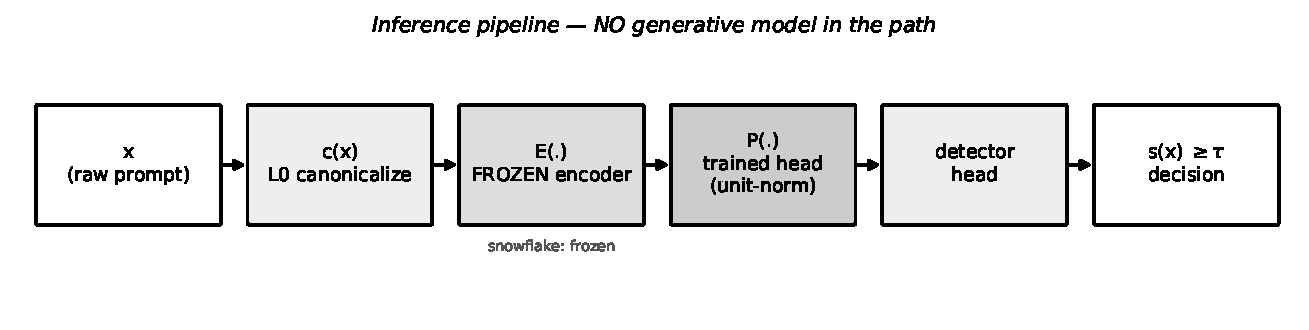
\includegraphics[width=\textwidth]{figures/canopi_architecture.pdf}
\caption{CANOPI inference pipeline. The canonicalizer and encoder are frozen; only
the projection head and the linear detector are trained. No generative model is on
the path.}\label{fig:arch}
\end{figure}

\subsection{Joint training objective}
Only $P$ and $(w,b)$ are trained. The loss couples four terms, each toggled by a
weight $\lambda_i$ (a term is off iff $\lambda_i=0$); the combination is the source
of CANOPI's behavior (Fig.~\ref{fig:joint}):
\begin{equation}
\mathcal{L} = \lambda_1\mathcal{L}_{\mathrm{inv}} + \lambda_2\mathcal{L}_{\mathrm{hard}} + \lambda_3\mathcal{L}_{\mathrm{drift}} + \lambda_4\mathcal{L}_{\mathrm{pAUC}} + \mathcal{L}_{\mathrm{BCE}}.
\end{equation}
$\mathcal{L}_{\mathrm{inv}}$ is a supervised-contrastive
loss~\cite{khosla2020supcon} over \emph{multiple views} of each anchor---paraphrase,
persona templating, encoding wraps, and NLLB-200 machine back-translations into a
diverse panel of languages (the cross-lingual positives)---pulling views that share
an intent together. $\mathcal{L}_{\mathrm{hard}}$ pushes attacks apart from benign
paraphrases that share a trigger token (e.g.\ ``ignore''). $\mathcal{L}_{\mathrm{drift}}$
regularizes $\lVert P(\canon(x))-P(\mathrm{view})\rVert$ across transform families.
$\mathcal{L}_{\mathrm{pAUC}}$ is a partial-AUC ``accuracy-at-the-top'' top-push
surrogate~\cite{macha2020deeptoppush,zhu2022pauc} that penalizes, for every positive,
the $\lceil\beta N_{\mathrm{neg}}\rceil$ hardest negatives---exactly the negatives
that set the $1\%$-FPR threshold ($\beta=0.01$)---so optimization targets the
deployment operating point rather than average separation. $\mathcal{L}_{\mathrm{BCE}}$
anchors the score scale. Views are training-time only; intent preservation is
enforced by an embedding-similarity filter and accept rates are logged. Baselines
are lambda settings of the same objective: B5 is the detector head alone
($\lambda_{1\text{--}4}=0$); B6 is invariance-only ($\lambda_4=0$); B7 is pAUC-only
($\lambda_{1\text{--}3}=0$).

\begin{figure}[t]\centering
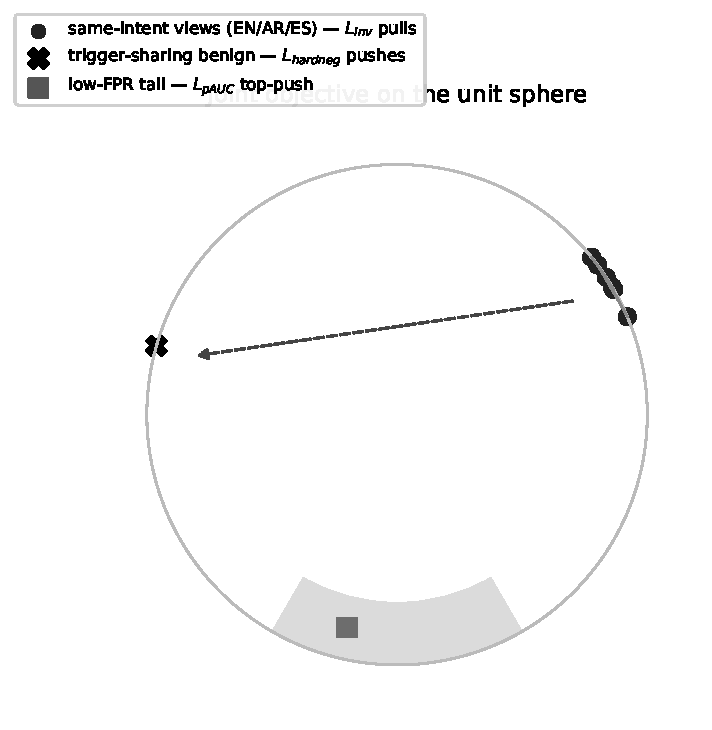
\includegraphics[width=0.62\textwidth]{figures/canopi_joint_objective.pdf}
\caption{The joint objective on the unit sphere: same-intent views (across
languages) are pulled together by $\mathcal{L}_{\mathrm{inv}}$, trigger-sharing
benign prompts are pushed away by $\mathcal{L}_{\mathrm{hard}}$, and the low-FPR
tail is optimized by $\mathcal{L}_{\mathrm{pAUC}}$.}\label{fig:joint}
\end{figure}

\subsection{Why the objective can substitute for---but not replace---a multilingual
encoder}\label{sec:method-boundary}
$P$ is a function of the \emph{frozen} features $E(\canon(x))$. The contrastive term
can only align two languages if $E$ maps them to representations that are
\emph{separable and consistent}: it learns a mapping from the encoder's
foreign-language region to the injection region, exploiting whatever structure $E$
already imposes on that language. When $E$ is multilingual, that structure is rich
and the alignment is already linearly available, so an invariance objective adds
little (the control). When $E$ is monolingual but still tokenizes a script into
informative sub-words (Latin scripts; substantial Chinese sub-word overlap), the
objective can recover the alignment the probe misses. When $E$ collapses a script to
near-uniform noise (Arabic, Devanagari, Cyrillic under an English encoder), no
training of $P$ can manufacture signal that is absent from its input. This predicts
the empirical boundary in Section~\ref{sec:results}.

\subsection{Evaluation protocol}\label{sec:protocol}
We reuse a fixed protocol for comparability. The primary corpus
(\texttt{xTRam1/safe-guard-prompt-injection}) is exact-deduplicated (SHA-256),
near-deduplicated (SimHash), and split $60/20/20$ stratified at seed $1337$ with an
empty train/val/test leakage report. The operating threshold $\tau$ is selected on
\emph{validation} at a $1\%$ FPR target and \emph{frozen} before any test read; no
per-corpus re-thresholding is permitted. The primary metric is $\Rfpr$. We report
mean$\pm$sd over five seeds $\{42,2025,7,1337,314\}$ with stratified bootstrap $95\%$
confidence intervals ($\ge\!500$ resamples). A difference ``matters'' only if its CI
excludes zero. We follow the adaptive-evaluation
norm~\cite{carlini2019eval,attackersecond2025}: an adaptive semantic-rewrite
adversary is reported as a recall-versus-strength curve, and the residual it leaves
is disclosed, not hidden.

% ============================================================
\section{Experimental Setup}\label{sec:setup}

\paragraph{Datasets.} In-domain: xTRam1 (above). Cross-lingual: a curated
Arabic/Spanish injection set (human-verified gold) plus a machine-translated
held-out panel obtained by translating English test positives into eight languages
spanning five scripts---Spanish, French, German, Portuguese (Latin), Chinese (Han),
Hindi (Devanagari), Russian (Cyrillic), and Arabic---via
NLLB-200~\cite{nllb2022}; these are held out from training and from $\tau$.
Cross-corpus: \texttt{deepset/prompt-injections} and JailbreakBench. Over-defense:
\texttt{leolee99/NotInject}.

\paragraph{Encoders.} The frozen $E$ is varied as the controlled factor:
\emph{multilingual} (\texttt{paraphrase-multilingual-MiniLM-L12-v2}) and
\emph{monolingual} (\texttt{all-MiniLM-L6-v2}, English). All else is held fixed.

\paragraph{Baselines.} B1 TF-IDF\,+\,LinearSVM; B2 ProtectAI DeBERTa-v3;
B3 InjecGuard; B5 plain embedding probe on $E(\canon(x))$ (the no-invariance floor);
B6 invariance-only; B7 pAUC-only. B2/B3 are loaded as published; cross-lingual
numbers for B2 are reported with the caveat that it over-triggers (its $\tau$
calibrates near zero, flagging all inputs) and so requires multilingual negatives
to interpret.

\paragraph{Implementation.} $P$ is a depth-2 MLP ($256\!\to\!128$, unit-norm);
$\lambda=(1,0.5,0.5,1)$, $\beta=0.01$, $30$ epochs, AdamW. Every experiment is one
YAML configuration; results are written to a fixed \texttt{runs/} layout with
per-seed checkpoints. One command reproduces each table and figure.

% ============================================================
\section{Results}\label{sec:results}

\subsection{The substitution result (primary)}\label{sec:res-mech}
Table~\ref{tab:mech} and Fig.~\ref{fig:mech} report the controlled encoder
ablation. On the \emph{monolingual} encoder the no-invariance probe B5 collapses
cross-lingually, while CANOPI recovers $\Rfpr$ by large margins whose $95\%$ CIs do
not overlap B5: French $0.12\!\to\!0.61$, Chinese $0.01\!\to\!0.51$, German
$0.02\!\to\!0.40$, Spanish-MT $0.23\!\to\!0.52$, Portuguese $0.18\!\to\!0.42$, and
curated Spanish $0.00\!\to\!0.22$. In-domain $\Rfpr$ is unchanged ($0.966\pm0.003$
vs.\ B5 $0.972$), so the cross-lingual ability is added at no in-domain cost. On the
\emph{multilingual} encoder CANOPI and B5 converge (Fig.~\ref{fig:mech}B), because
the encoder already supplies the alignment. The objective therefore substitutes for
multilingual pretraining precisely where the encoder lacks the languages, answering
RQ1 and RQ2.

\begin{table}[t]\centering
\caption{Substitution result---monolingual encoder, $\Rfpr$ (mean$\pm$sd, 5 seeds).
B5 is the no-invariance probe on the same frozen features. $^{*}$ MT-translated
held-out test set. Recovery is CI-separated for the top block; the bottom block is
the boundary (Section~\ref{sec:method-boundary}).}\label{tab:mech}
\begin{tabular}{lccc}
\toprule
Language & CANOPI & B5 (no-inv.) & $\Delta$ \\
\midrule
French$^{*}$  & $0.61\pm0.06$ & $0.12\pm0.00$ & $+0.49$ \\
Chinese$^{*}$ & $0.51\pm0.13$ & $0.01\pm0.00$ & $+0.49$ \\
German$^{*}$  & $0.40\pm0.10$ & $0.02\pm0.00$ & $+0.38$ \\
Spanish$^{*}$ & $0.52\pm0.05$ & $0.23\pm0.00$ & $+0.29$ \\
Portuguese$^{*}$ & $0.42\pm0.04$ & $0.18\pm0.00$ & $+0.24$ \\
Spanish (curated) & $0.22\pm0.07$ & $0.00\pm0.00$ & $+0.22$ \\
\midrule
Arabic & $0.01\pm0.02$ & $0.00\pm0.00$ & $\approx 0$ \\
Hindi$^{*}$ & $0.02\pm0.02$ & $0.00\pm0.00$ & $\approx 0$ \\
Russian$^{*}$ & $0.01\pm0.00$ & $0.00\pm0.00$ & $\approx 0$ \\
\midrule
In-domain (English) & $0.966\pm0.003$ & $0.972\pm0.000$ & $-0.006$ \\
\bottomrule
\end{tabular}
\end{table}

\begin{figure}[t]\centering
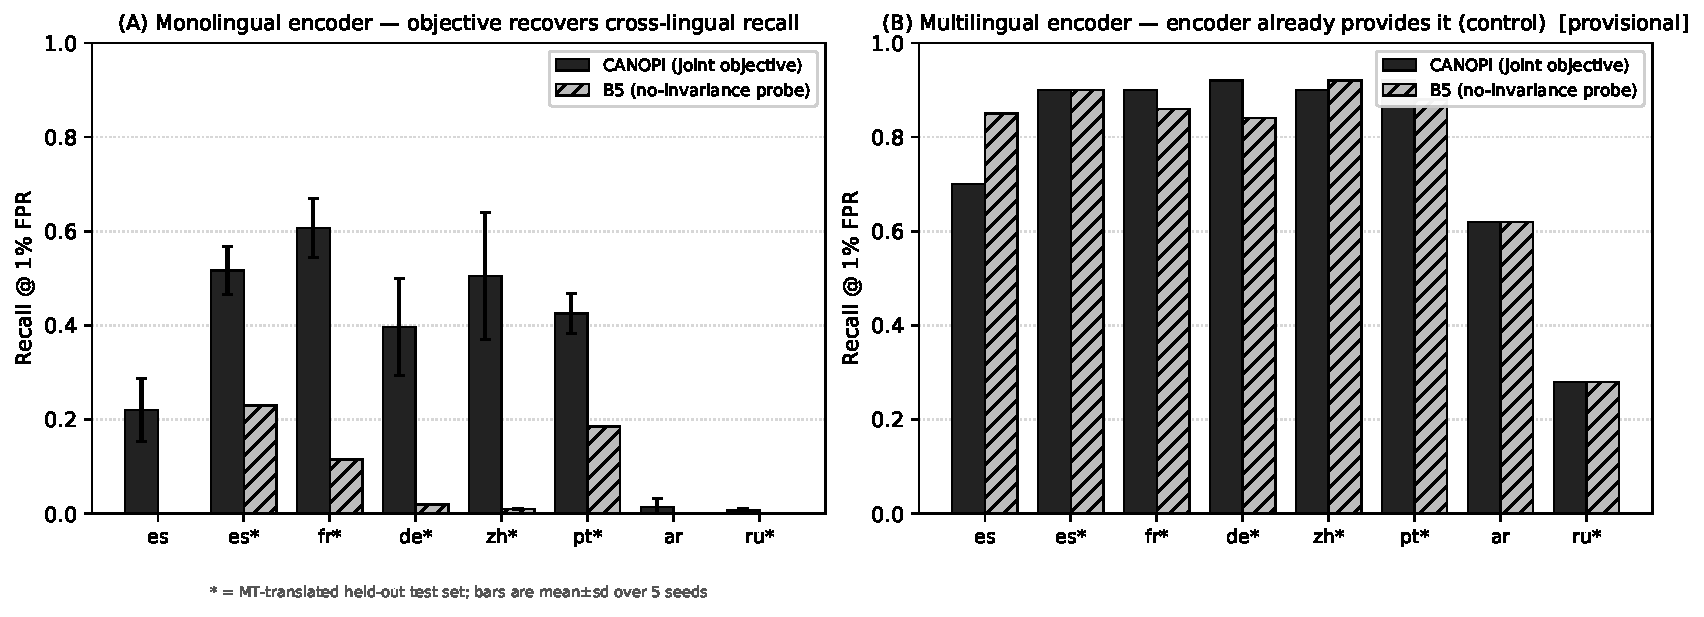
\includegraphics[width=\textwidth]{figures/canopi_mechanism.pdf}
\caption{The encoder $\times$ objective mechanism. \textbf{(A)} Monolingual encoder:
the no-invariance probe B5 collapses cross-lingually; CANOPI's invariance objective
recovers it (5 seeds, mean$\pm$sd). \textbf{(B)} Multilingual encoder: the two
converge---the control that localizes the objective's value. Panel~B is provisional
pending the full five-seed run.}\label{fig:mech}
\end{figure}

\subsection{The boundary}\label{sec:res-boundary}
The languages CANOPI does \emph{not} recover on the English encoder---Arabic, Hindi,
Russian (bottom block of Table~\ref{tab:mech})---are exactly the non-Latin scripts
that encoder tokenizes to near-uniform features. This is the predicted boundary of
Section~\ref{sec:method-boundary}: invariance amplifies weak-but-present signal but
cannot create it. Natural romanized Arabic remains an open case (B5 $0.20$ vs.\
CANOPI $0.09$), the one bucket the probe wins, and we report it as such (RQ3).

\subsection{Attribution: invariance, not the operating-point term}\label{sec:res-attr}
To attribute the recovery to the invariance machinery rather than the partial-AUC
term, we evaluate invariance-only (B6, $\lambda_4\!=\!0$) on the monolingual encoder
(five seeds). Invariance-only \emph{reproduces} the lift: it recovers $\Rfpr$ far
above the probe B5 on the same languages---Spanish-MT $0.59\!\pm\!0.05$ (B5 $0.23$),
Portuguese $0.55\!\pm\!0.07$ ($0.18$), French $0.52\!\pm\!0.12$ ($0.12$), German
$0.30\!\pm\!0.10$ ($0.02$), curated Spanish $0.23\!\pm\!0.13$ ($0.00$)---matching
full CANOPI on the Latin-script languages. Removing the partial-AUC term therefore
does not remove the recovery, so the operating-point term is not its source. The two
terms are nonetheless not redundant: on Chinese the pAUC term contributes
substantially ($0.15$ invariance-only vs.\ $0.51$ full CANOPI). The complementary
pAUC-only run (B7, $\lambda_{1\text{--}3}\!=\!0$, no invariance views), pre-registered
to stay collapsed, completes the dissociation \emph{[pending]}.

\subsection{In-domain and operating-point behavior}\label{sec:res-op}
\emph{[PROVISIONAL---smoke pass (seed 42); full five-seed run pending.]} In-domain,
CANOPI is competitive at the strict operating point (provisional $\Rfpr=0.92$, vs.\
B5 $0.90$, B1 $0.98$; the corpus is near-saturated at $1\%$ FPR). We also
pre-registered, before the run, an operating-point-robustness hypothesis: that the
joint objective would beat B5 on threshold transfer, over-defense, and adaptive
robustness. The smoke pass does \emph{not} support it---B5 matches or slightly beats
CANOPI on over-defense and adaptive robustness---and we report this honestly; the
contribution of this paper is the substitution result, not operating-point
superiority. Final five-seed numbers and confidence intervals will replace this
paragraph.

% ============================================================
\section{Discussion}\label{sec:discussion}

\paragraph{Pretraining versus a training objective.} The substitution result reframes
a design choice. Cross-lingual injection detection is usually pursued by scaling the
encoder (multilingual pretraining) or by adding an inference-time LLM. We show a
third axis: a training-time invariance objective can buy the same cross-lingual
recall on a smaller, English encoder, where it is otherwise absent, with no
inference-time cost. The multilingual-encoder control is essential to the claim---it
is what turns ``CANOPI does well cross-lingually'' into ``the objective, not the
encoder, is responsible,'' by exhibiting the regime where the two coincide.

\paragraph{When it provably cannot help.} The boundary is not a failure but a
characterization: a frozen encoder defines the information available to $P$, and
invariance training is an amplifier, not a source. For scripts the encoder discards,
the honest remedies are an encoder that represents them or a transliteration pivot
in $\canon$---both orthogonal to the objective.

\paragraph{Limitations.} (i)~The multilingual-encoder control and the in-domain and
operating-point numbers are reported from a smoke pass and will be finalized at five
seeds. (ii)~Absolute recovered recall is moderate ($0.40$--$0.61$ on the best
languages), not near-ceiling; the objective narrows, not closes, the gap to a
multilingual encoder. (iii)~Non-Latin scripts on an English encoder, and natural
romanized text, are not recovered. (iv)~A semantic-rewrite adversary leaves an
irreducible residual that canonicalization cannot remove, which we report rather
than hide.

% ============================================================
\section{Conclusion}\label{sec:conclusion}
We presented CANOPI, a no-LLM prompt-injection detector whose projection head learns
cross-lingual invariance over a frozen canonicalizer and encoder. Through a
controlled encoder ablation we showed that the invariance objective substitutes for
multilingual pretraining: it recovers cross-lingual Recall at $1\%$ FPR that a linear
probe loses on a monolingual encoder, at no in-domain cost, and converges with the
probe when the encoder is already multilingual---localizing the objective's value to
where the encoder lacks the languages, within a boundary set by what the encoder
represents. The result offers a cheaper, deterministic alternative to multilingual
or LLM-based guardrails for the languages an encoder can see, and a precise account
of where that alternative stops working.

% ============================================================
\section*{Declarations}
\noindent\textbf{Funding.} Not applicable.\\
\textbf{Conflict of interest.} The authors declare no competing interests.\\
\textbf{Ethics approval.} Not applicable.\\
\textbf{Consent to participate / for publication.} Not applicable.\\
\textbf{Data availability.} All primary datasets are public (xTRam1, deepset,
NotInject, JailbreakBench); the curated and machine-translated multilingual
evaluation sets are released with the code.\\
\textbf{Code availability.} Code, configurations, and per-seed run logs:
\url{https://github.com/ShaikhaTheGreen/HybridGuard}.\\
\textbf{Author contributions.} S.A.\ designed the method and experiments and wrote
the manuscript; H.A.\ and A.A.\ contributed to the evaluation and data curation. All
authors reviewed the manuscript.\\
\textbf{Reproducibility note.} Malicious prompts are never logged verbatim
(safe-excerpting); the primary result is pre-registered with a frozen operating
point.

\bibliography{references_npl}

\end{document}
